\input{../preamble.tex}
\SetDate[15/04/2026]
\setbeamertemplate{page number in head/foot}{}

\begin{document}

\section{Automatismes}

\begin{frame}

\centering \huge
Automatismes

\large
Calculatrice interdite

\end{frame}

\subsection{Équations}

\framedelayed{
	Donner le $x\in\R, x\neq0,$ vérifiant l'équation suivante.
	\boxBA{
		$\dfrac8x  =\dfrac{\sqrt{3}}2$
	}{
		$\dfrac3x = \dfrac12$
	}
}{
	\boxBA{
		$\dfrac8x  =\dfrac{\sqrt{3}}2 \iff x = \dfrac{2\times8}{\sqrt3} = \dfrac{16}3\sqrt3$
	}{
		$\dfrac3x = \dfrac12 \iff x = 3\times2 = 6$
	}
}


\framedelayed{
	Donner le $x\in\R, x\neq0,$ vérifiant l'équation suivante.
	\boxBA{
		$\dfrac7x  =\dfrac12$
	}{
		$\dfrac2x =\sqrt{3}$
	}
}{
	\boxBA{
		$\dfrac7x  =\dfrac12 \iff x = 7\times2 = 14$
	}{
		$\dfrac2x =\sqrt{3} \iff x = \dfrac2{\sqrt3} = \dfrac23\sqrt3$
	}
}


\subsection{Trigonométrie}

\framedelayed{
	Calculer la longueur \textbf{exacte} de $AC$.

	\begin{tcbraster}[raster columns=2,raster equal height,nobeforeafter,raster column skip=1cm]
	\boxBA{
		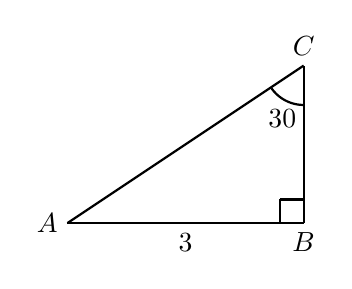
\begin{tikzpicture}[scale=1]
			\draw[-, thick, black] (0,0) -- (3,0) node[midway, below] {$3$};
			\draw[-, thick, black] (3,0) -- (3,2);
			\draw[-, thick, black] (3,2) -- (0,0);
			
			\node[black, left] at  (0,0) {$A$};
			\node[black, below] at  (3,0) {$B$};
			\node[black, above] at  (3,2) {$C$};
			% angle droit
			\draw[-, thick, black] (3,.3)-- (2.7,.3);
			\draw[-, thick, black] (2.7,.3)-- (2.7,0);
			
			% angle
			\draw [black,thick,domain=215:270] plot ({3+.5*cos(\x)}, {2+.5*sin(\x)})
			node[below=5pt, left=-1pt] {$30\degree$};
		\end{tikzpicture}
	}{
		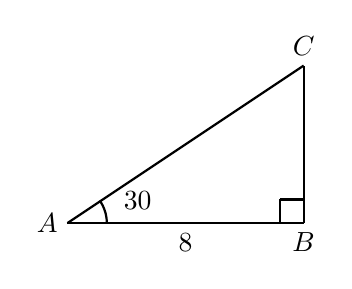
\begin{tikzpicture}[scale=1]
			\draw[-, thick, black] (0,0) -- (3,0) node[midway, below] {$8$};
			\draw[-, thick, black] (3,0) -- (3,2);
			\draw[-, thick, black] (3,2) -- (0,0);
			
			\node[black, left] at  (0,0) {$A$};
			\node[black, below] at  (3,0) {$B$};
			\node[black, above] at  (3,2) {$C$};
			% angle droit
			\draw[-, thick, black] (3,.3)-- (2.7,.3);
			\draw[-, thick, black] (2.7,.3)-- (2.7,0);
			
			% angle
			\draw [black,thick,domain=0:35] plot ({.5*cos(\x)}, {.5*sin(\x)})
			node[left=5pt, right=10pt] {$30\degree$};
		\end{tikzpicture}
	}
	\end{tcbraster}
	
	$\sin(30\degree) = \dfrac12,$
	$\cos(30\degree) = \dfrac{\sqrt{3}}2,$ et $\tan(30\degree) = \dfrac1{\sqrt{3}}.$
}{
	\begin{tcbraster}[raster columns=2,raster equal height,nobeforeafter,raster column skip=1cm]
	\boxBA{
		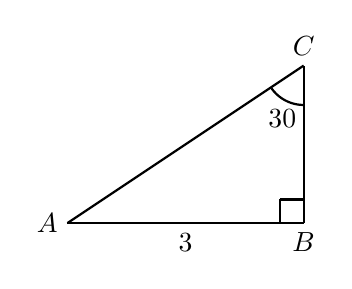
\begin{tikzpicture}[scale=1]
			\draw[-, thick, black] (0,0) -- (3,0) node[midway, below] {$3$};
			\draw[-, thick, black] (3,0) -- (3,2);
			\draw[-, thick, black] (3,2) -- (0,0);
			
			\node[black, left] at  (0,0) {$A$};
			\node[black, below] at  (3,0) {$B$};
			\node[black, above] at  (3,2) {$C$};
			% angle droit
			\draw[-, thick, black] (3,.3)-- (2.7,.3);
			\draw[-, thick, black] (2.7,.3)-- (2.7,0);
			
			% angle
			\draw [black,thick,domain=215:270] plot ({3+.5*cos(\x)}, {2+.5*sin(\x)})
			node[below=5pt, left=-1pt] {$30\degree$};
		\end{tikzpicture}
		\begin{align*}
			\sin(30\degree) = \dfrac12 = \dfrac{3}{AC} \\
			AC = 2\times3 = 6
		\end{align*}
	}{
		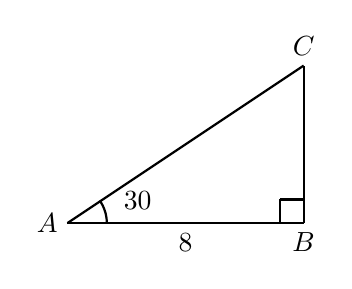
\begin{tikzpicture}[scale=1]
			\draw[-, thick, black] (0,0) -- (3,0) node[midway, below] {$8$};
			\draw[-, thick, black] (3,0) -- (3,2);
			\draw[-, thick, black] (3,2) -- (0,0);
			
			\node[black, left] at  (0,0) {$A$};
			\node[black, below] at  (3,0) {$B$};
			\node[black, above] at  (3,2) {$C$};
			% angle droit
			\draw[-, thick, black] (3,.3)-- (2.7,.3);
			\draw[-, thick, black] (2.7,.3)-- (2.7,0);
			
			% angle
			\draw [black,thick,domain=0:35] plot ({.5*cos(\x)}, {.5*sin(\x)})
			node[left=5pt, right=10pt] {$30\degree$};
		\end{tikzpicture}
		\begin{align*}
			\cos(30\degree) = \dfrac{\sqrt3}2 = \dfrac{8}{AC} \\
			AC = \dfrac{2\times8}{\sqrt3} = \dfrac{16}3\sqrt3
		\end{align*}
	}
	\end{tcbraster}
}



\framedelayed{
	Calculer la longueur \textbf{exacte} de $AB$.

	\begin{tcbraster}[raster columns=2,raster equal height,nobeforeafter,raster column skip=1cm]
	\boxBA{
		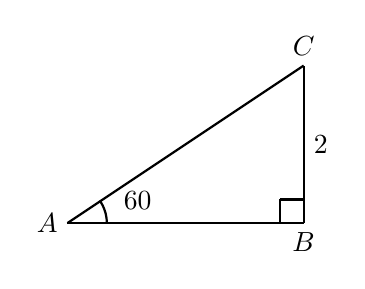
\begin{tikzpicture}[scale=1]
			\draw[-, thick, black] (0,0) -- (3,0);
			\draw[-, thick, black] (3,0) -- (3,2)  node[midway, right] {$2$} ;
			\draw[-, thick, black] (3,2) -- (0,0);
			
			\node[black, left] at  (0,0) {$A$};
			\node[black, below] at  (3,0) {$B$};
			\node[black, above] at  (3,2) {$C$};
			% angle droit
			\draw[-, thick, black] (3,.3)-- (2.7,.3);
			\draw[-, thick, black] (2.7,.3)-- (2.7,0);
			
			% angle
			\draw [black,thick,domain=0:35] plot ({.5*cos(\x)}, {.5*sin(\x)})
			node[left=5pt, right=10pt] {$60\degree$};
		\end{tikzpicture}
	}{
		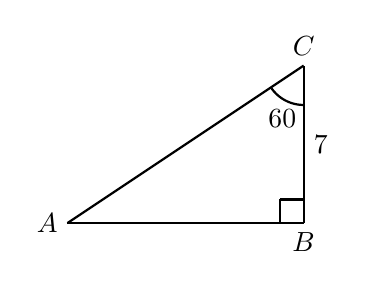
\begin{tikzpicture}[scale=1]
			\draw[-, thick, black] (0,0) -- (3,0);
			\draw[-, thick, black] (3,0) -- (3,2) node[midway, right] {$7$} ;
			\draw[-, thick, black] (3,2) -- (0,0);
			
			\node[black, left] at  (0,0) {$A$};
			\node[black, below] at  (3,0) {$B$};
			\node[black, above] at  (3,2) {$C$};
			% angle droit
			\draw[-, thick, black] (3,.3)-- (2.7,.3);
			\draw[-, thick, black] (2.7,.3)-- (2.7,0);
			
			% angle
			\draw [black,thick,domain=215:270] plot ({3+.5*cos(\x)}, {2+.5*sin(\x)})
			node[below=5pt, left=-1pt] {$60\degree$};
		\end{tikzpicture}
	}
	\end{tcbraster}

	$\cos(60\degree) = \dfrac12,$
	$\sin(60\degree) = \dfrac{\sqrt{3}}2,$ et $\tan(60\degree) =\sqrt{3}.$
}{
	\begin{tcbraster}[raster columns=2,raster equal height,nobeforeafter,raster column skip=1cm]
	\boxBA{
		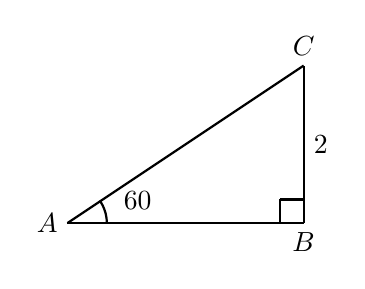
\begin{tikzpicture}[scale=1]
			\draw[-, thick, black] (0,0) -- (3,0);
			\draw[-, thick, black] (3,0) -- (3,2)  node[midway, right] {$2$} ;
			\draw[-, thick, black] (3,2) -- (0,0);
			
			\node[black, left] at  (0,0) {$A$};
			\node[black, below] at  (3,0) {$B$};
			\node[black, above] at  (3,2) {$C$};
			% angle droit
			\draw[-, thick, black] (3,.3)-- (2.7,.3);
			\draw[-, thick, black] (2.7,.3)-- (2.7,0);
			
			% angle
			\draw [black,thick,domain=0:35] plot ({.5*cos(\x)}, {.5*sin(\x)})
			node[left=5pt, right=10pt] {$60\degree$};
		\end{tikzpicture}
		\begin{align*}
			\tan(60\degree) = \sqrt3 = \dfrac{2}{AB} \\
			AB = \dfrac2{\sqrt3} = \dfrac23\sqrt3
		\end{align*}
	}{
		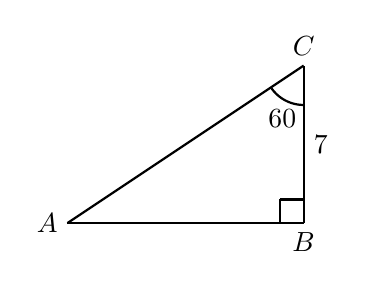
\begin{tikzpicture}[scale=1]
			\draw[-, thick, black] (0,0) -- (3,0);
			\draw[-, thick, black] (3,0) -- (3,2) node[midway, right] {$7$} ;
			\draw[-, thick, black] (3,2) -- (0,0);
			
			\node[black, left] at  (0,0) {$A$};
			\node[black, below] at  (3,0) {$B$};
			\node[black, above] at  (3,2) {$C$};
			% angle droit
			\draw[-, thick, black] (3,.3)-- (2.7,.3);
			\draw[-, thick, black] (2.7,.3)-- (2.7,0);
			
			% angle
			\draw [black,thick,domain=215:270] plot ({3+.5*cos(\x)}, {2+.5*sin(\x)})
			node[below=5pt, left=-1pt] {$60\degree$};
		\end{tikzpicture}
		\begin{align*}
			\tan(60\degree) = \sqrt3 = \dfrac{AB}{7} \\
			AB = 7\sqrt3
		\end{align*}
	}
	\end{tcbraster}
}



\section{Solutions}

\shipoutAnswer

\end{document}